\section{Results and Evaluation}

One of the objectives of this project is to react to events, which is why recent information is crucial to all of the models developed. Consider the two contrasting examples: 1) if there has been a collision on the road, all buses that use this route will be delayed compared to 2) if a bus driver is in an argument with one of the passengers getting on the bus, then only that particular bus would be delayed, not any of the other buses on the route. In the first case, the desired outcome is indeed to react to this increase in journey time and provide predictions with longer than usual journey times. However, in the second case, the `delay' is localised to that particular bus and so predictions should not provide predictions with longer than usual journey times. Therefore, it is possible to overreact to situations and adjust the prediction when there is not an actual cause for the model to do so. \\

In the context of bus journey times, the mean absolute error (MAE) and the root mean squared error (RMSE) mean different things and provide different insights. The MAE results describe how many seconds off the actual journey time a model consistently predicts. For example, an MAE of 100 seconds implies that the model consistently predicts a journey time of 100 seconds more or less than the actual journey time (although it does not provide insight into whether the model over or under predicts). On the other hand, since the errors are squared before they are averaged, the RMSE gives a relatively high weight to large errors. This penalization of large errors could be appropriate if for example, a prediction that is four minutes off is more than twice as bad as a prediction that is two minutes off. This brings to question, what counts as a `good' bus journey prediction? \\ 

So, is a model that predicts journeys that are consistently 3 minutes off better than a model that predicts journeys that are 1 minute off occasionally and 5 minutes off occasionally? In the long run, waiting an extra minute or two doesn't make much of a difference. However, waiting upwards of 5 minutes is significant. This suggests that the RMSE results are more important than the MAE results. On the other hand, if waiting 5 extra minutes is no more than twice as bad as waiting around 2 extra minutes, then the MAE is actually more appropriate. Therefore since this is a fairly subjective issue, for this project, both the MAE and RMSE will be presented. 

\subsection{Historical Model}

First consider the results for journeys between stops that are five apart. \\

Figure \ref{fig:historical-past2hours} shows the predicted journey time versus the actual journey time versus TfL's own predicted journey time. This figure is for buses on route 52 for journeys between Chesterton Road to Notting Hill Gate Station, where the predictions have been found using the historical model that looks back at buses in the past two hours. 

\begin{figure}[H]
\begin{center}
    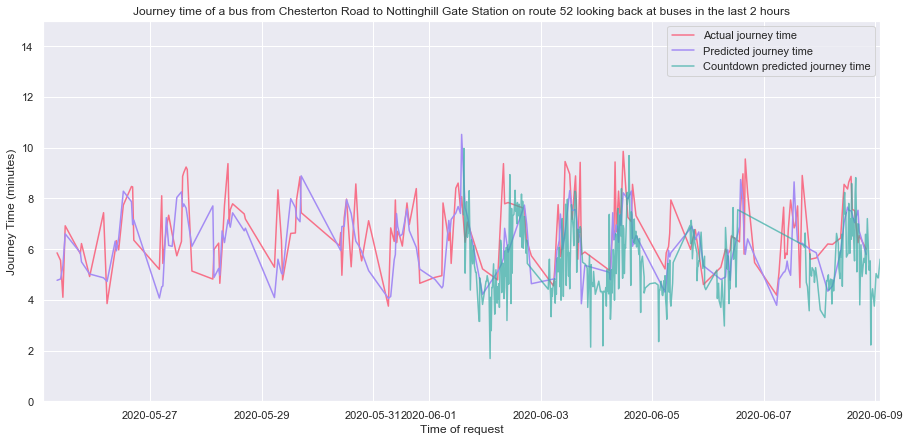
\includegraphics[keepaspectratio, width=15cm]{Images/historical-past2hours.png}
    \caption{Historical Model looking at buses from past two hours}
    \label{fig:historical-past2hours}
\end{center}
\end{figure}

Graphs such as in Figure \ref{fig:historical-past2hours} were also produced for predictions that were found using the historical models that looked back at the past 15 minutes, 30 minutes and 60 minutes. The MAE and RMSE were calculated for all four models that look back X amount of time. The results can be seen in Figure \ref{fig:historical-lookingbacktime}. 

\begin{figure}[H]
\begin{center}
    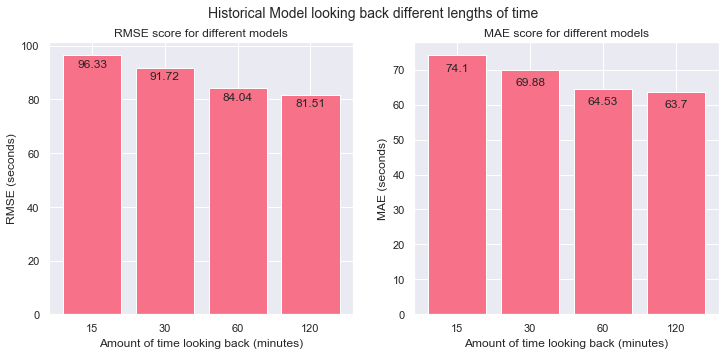
\includegraphics[keepaspectratio, width=15cm]{Images/historical-amountoftime-gap5.png}
    \caption{Historical Model looking back at x amount of time}
    \label{fig:historical-lookingbacktime}
\end{center}
\end{figure}

Consider the model that looks back at journeys from the past 120 minutes. Figure \ref{fig:historical-lookingbacktime} indicates that based on the MAE, the predictions are on average about a minute higher or lower than the actual journey time. This is an excellent result, however, bear in mind that this is only for stops that are five apart. It will be shown later that when these models are applied to stops that are further apart, the MAE and RMSE grow. Since the RMSE is only about 20 seconds more than the MAE, this suggests that either predictions that are significantly off don't occur very often or predictions are generally close to 1 minute off. \\

Intuitively, it makes sense that the model that looks back at the last 15 minutes performs the worst out of the four sub-models presented above. This is because looking at only the past 15 minutes means the probability of overreacting to an event is much higher. In particular, Figure \ref{fig:historical-past2hours} demonstrates that the actual journey time ranges between 4 minutes to 10 minutes and so when the model looks back at the last 15 minutes, it will be looking at most at the last three buses. In the worst case, it would only look back at the last bus. This means that if there is something that causes only that particular bus to delay, the model will not realise that this is an anomalous journey time and so will predict a longer journey time when it should not have. \\

Figure \ref{fig:historical-past2buses} shows the predicted journey time versus the actual journey time versus TfL's own predicted journey time. This figure is also for buses on route 52 for journeys between Chesterton Road to Notting Hill Gate Station. However, here the predictions have been found using the historical model that looks back at the last two buses to complete the journey.

\begin{figure}[H]
\begin{center}
    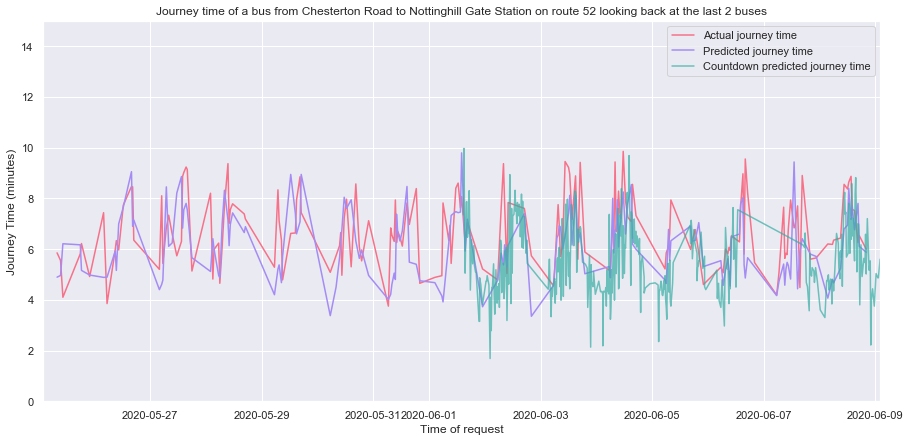
\includegraphics[keepaspectratio, width=15cm]{Images/historical-past2buses.png}
    \caption{Historical Model looking at past two buses}
    \label{fig:historical-past2buses}
\end{center}
\end{figure}

Graphs such as in Figure \ref{fig:historical-past2buses} were also produced for predictions that were found using the historical models that looked back at the past 5 buses, 10 buses and 15 buses. The MAE and RMSE were calculated and can be seen in Figure \ref{fig:historical-lookingbackbuses}.

\begin{figure}[H]
\begin{center}
    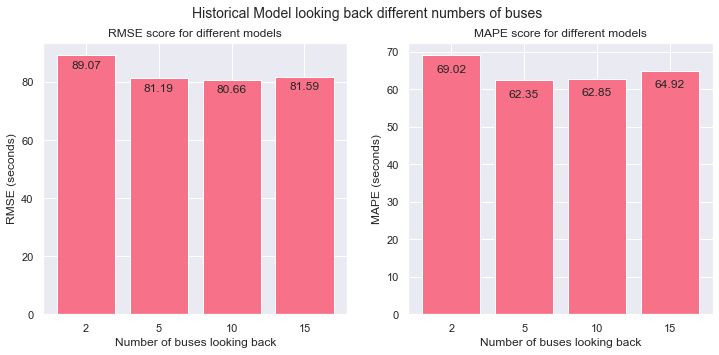
\includegraphics[keepaspectratio, width=15cm]{Images/historical-numberofbuses-gap5.png}
    \caption{Historical Model looking back at x number of buses}
    \label{fig:historical-lookingbackbuses}
\end{center}
\end{figure}

Consider the model that looks back at the last five buses. Based on the MAE, Figure \ref{fig:historical-lookingbackbuses} implies that predictions are on average about a minute more or less than the actual journey time. However, as before, these are results for bus stops that are five apart and so should not be treated as conclusive results. \\

In a similar argument to earlier, it makes sense for the model that looks back at the last two buses to perform the worst out of the four sub-models presented above. This is because of its high probability of overreacting to events. On the other hand, it also makes sense that the model that looks back at the last 15 buses doesn't perform as well as the one that looks back at the last 5 or 10 buses. This is because this model is more likely to take journey times that are no longer relevant into account. For example, consider the following case: a bus is not a 24 hour bus route - its last bus is at 00:30 and its first bus is at 05:25. If a prediction is requested at 05:40, the last 15 buses will include bus journeys made around midnight or before. As mentioned in Section \ref{section:data-exploration}, at different times of day the journey times are not the same. Therefore, the prediction could be less than it should be. Furthermore, if there was some disruption that caused the bus journeys around midnight to be significantly longer or shorter, this too could adversely affect the prediction. However, since its performance is not actually significantly worse than the model that looks back at the last 5 or 10 buses, this could be put down to the weights that were chosen that ensured that bus journeys long before the request time do not have as much impact on the prediction. \\

Figure \ref{fig:historical-gap5-all-compare} shows all eight sub-models' MAE and RMSE for stops that are five apart compared against each other. According to the RMSE the best two models are 1) looking back 10 buses 2) looking back 5 buses. According to the MAE the best two models are 1) looking back 5 buses 2) looking back 10 buses. Overall, this means that the top two sub-models, found by averaging the MAE and RMSE are 1) looking back 10 buses 2) looking back 5 buses. The third and fourth best sub-models overall are 3) looking back 2 hours 4) looking back 15 buses. 

\begin{figure}[H]
\begin{center}
    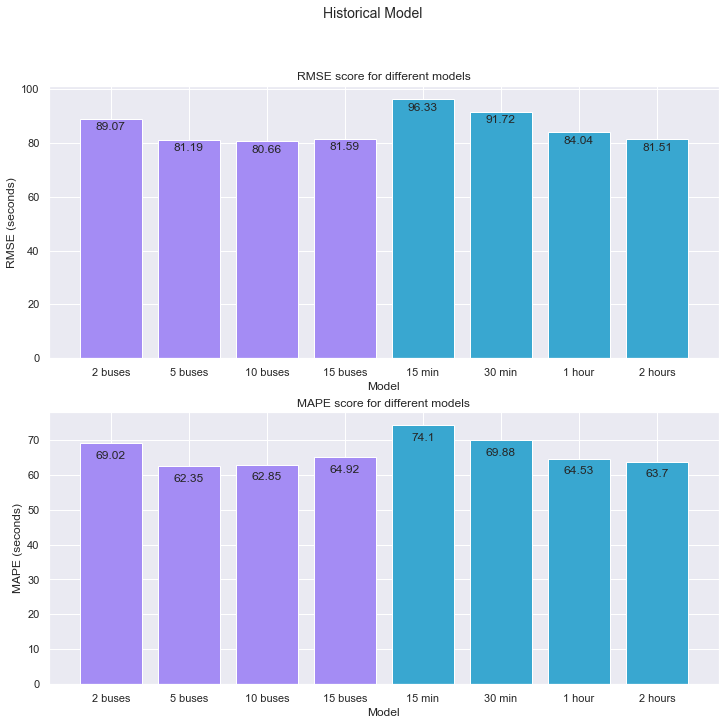
\includegraphics[keepaspectratio, width=15cm]{Images/historical-all-compare-gap5.png}
    \caption{Historical Model}
    \label{fig:historical-gap5-all-compare}
\end{center}
\end{figure}

Figure \ref{fig:historical-gap5-all-compare} shows that the models that look back a certain amount of time have a larger range than the models that look back a certain amount of time. This suggests that the models that look back a certain amount of time are more likely to produce predictions that are further away from the actual value. Therefore, it can be concluded that looking back a specified number of buses is more likely to produce better results than looking back a specified amount of time. The ranges are as follows:

\begin{itemize}
    \item Historical model looking back different amounts of time: RMSE range = 14.82 seconds, MAE range = 10.4 seconds.
    \item Historical model looking back different numbers of buses: RMSE range = 8.41 seconds, MAE range = 6.67 seconds.
\end{itemize}

The best two models were applied to pairs of stops that are larger than five apart. The results for the model that looks back 10 stops are seen in Figure INSERT and the results for the model that looks back 5 stops are seen in Figure INSERT. \\

INSERT FIGURE \\

It can be seen that for both models as the distance between the stops grow, so too does the RMSE and MAE. This makes sense because as the stops grow further apart, the standard deviation and variance of the actual journey times also increase. This means that there is a lot more fluctuation in the training times given to the models to calculate a weighted average out of. \\

Based on gaps of all sizes, the best overall historical model is TODO \\ 

TODO: Conclusions about 

\subsection{Regression + Interpolation Model}

TODO: Presents results for all gaps (not just gap of 5 like with historical). 

\begin{figure}[H]
\begin{center}
    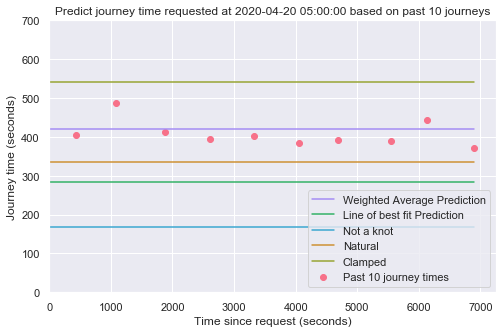
\includegraphics[keepaspectratio, width=14cm]{Images/regression-part2-comparison.png}
    \caption{Regression model prediction comparison}
    \label{fig:regression-comparison}
\end{center}
\end{figure}

\begin{figure}[H]
\begin{center}
    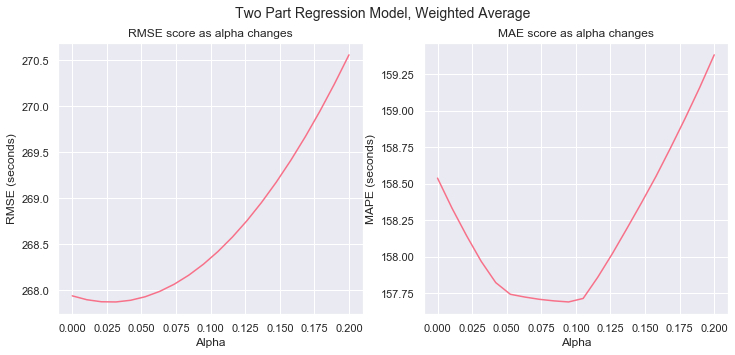
\includegraphics[keepaspectratio, width=14cm]{Images/regression-combined-weightedavg.png}
    \caption{Part 2 = Weighted Average}
    \label{fig:regression-part2weightedavg}
\end{center}
\end{figure}

\begin{figure}[H]
\begin{center}
    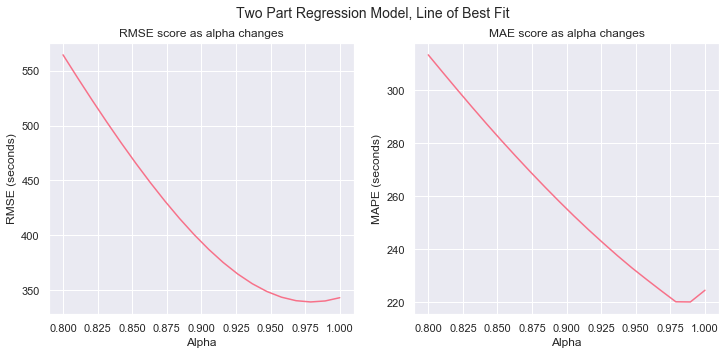
\includegraphics[keepaspectratio, width=14cm]{Images/regression-combined-lineofbestfit.png}
    \caption{Part 2 = Line of Best Fit}
    \label{fig:regression-part2lineofbestfit}
\end{center}
\end{figure}

TODO: Makes sense for cubic splines to bad 

\begin{figure}[H]
\begin{center}
    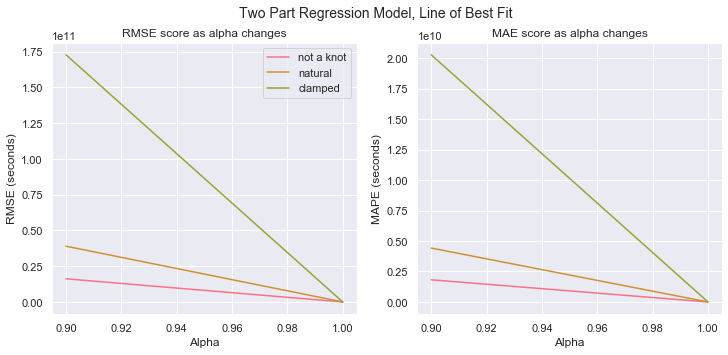
\includegraphics[keepaspectratio, width=14cm]{Images/regression-combined-cubicspline.png}
    \caption{Part 2 = Cubic Spline}
    \label{fig:regression-part2cubicspline}
\end{center}
\end{figure}

TODO: Talk about how expected alpha to be in the region of 0.5. Explain what it means for alpha to be at those extreme values and how that supports or corroborates the hypotheses.

\begin{figure}[H]
\begin{center}
    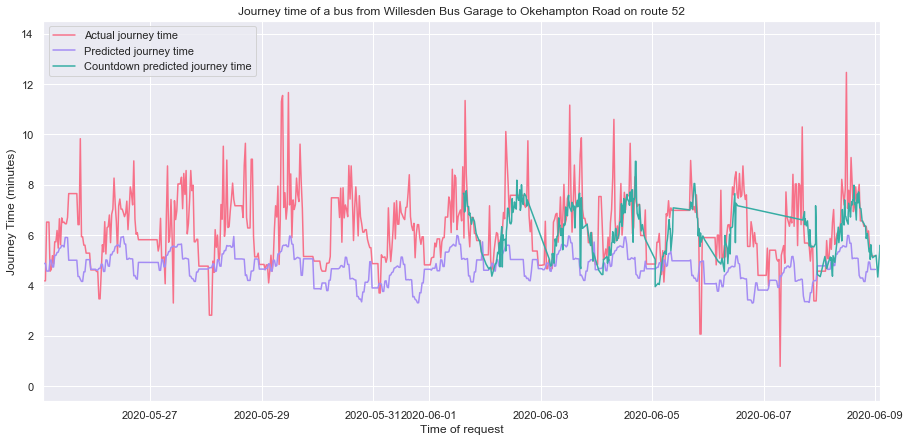
\includegraphics[keepaspectratio, width=15cm]{Images/regression-journey-comparison.png}
    \caption{Regression Model}
    \label{fig:regression-gap5-journey-comparison}
\end{center}
\end{figure}

\begin{figure}[H]
\begin{center}
    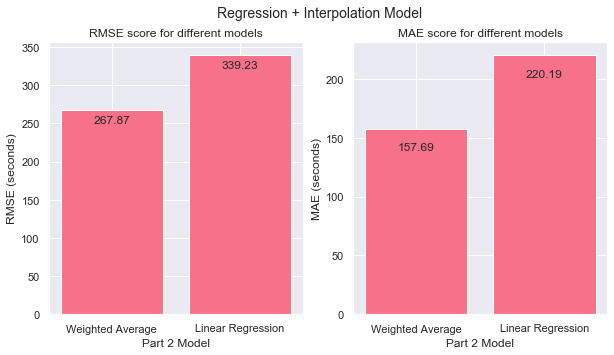
\includegraphics[keepaspectratio, width=12cm]{Images/regression-comparison-allgaps.png}
    \caption{All Gap size comparison}
    \label{fig:regression-comparison-allgaps}
\end{center}
\end{figure}

\subsection{Cross Model Comparison}

In order for the models to be compared directly, it was necessary for \\

TODO: Talk about the MAE and RMSE mean in the context of bus journey times i.e. the thing about like predictions being consistently 3 mintues off versus predictions occasionally being 1 minute off and occasionally 5 minutes off.

\begin{figure}[H]
\begin{center}
    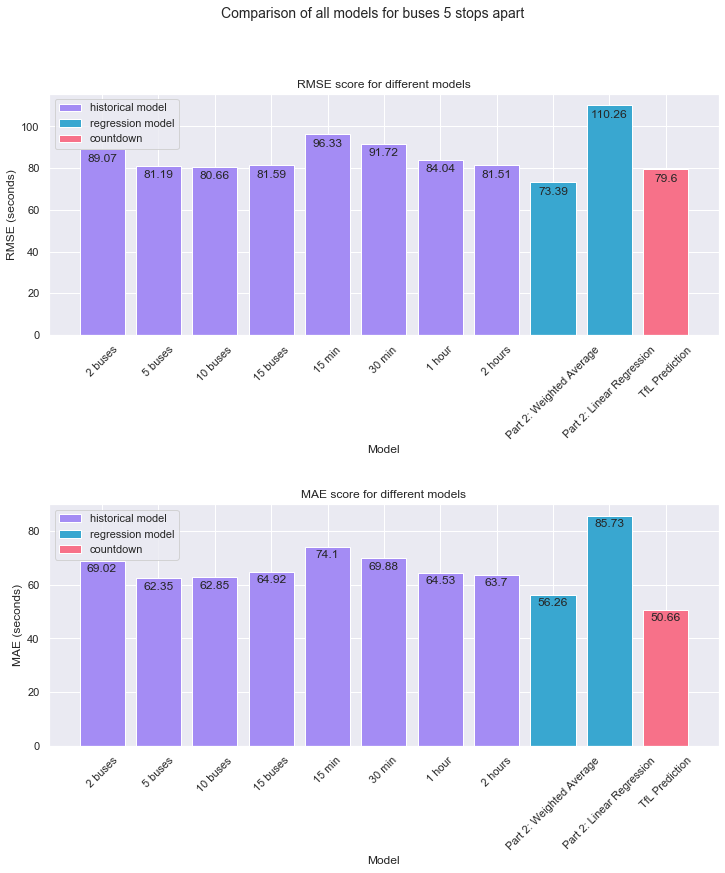
\includegraphics[keepaspectratio, width=15cm]{Images/evaluation-all-comparison-gap5.png}
    \caption{All Model Comparison}
    \label{fig:all-model-comparison}
\end{center}
\end{figure}

\subsection{Future Work + Improvements}

Currently, the models developed in this project are only compared against each other and against TfL Countdown's own predictions. None of the models made use of traffic conditions and it has been assumed that Countdown also does not look at factors such as congestion. On the other hand, other applications such as CityMapper or Google Maps provide adjustable predicted journey times based on traffic conditions. So, in the future, it would be interesting to see a direct comparison of this project's models against CityMapper and Google Map's predictions. This should provide insight into whether traffic conditions is necessary for vehicle journey predictions. \\

Artificial Neural Networks were a type of model that was not prioritised for this project. However, given more time, it would be interesting to see how an ANN model would compare to the historical average and regression + interpolation combined model. \\

\clearpage